\section{Progettazione}
Nella fase iniziale, il gruppo ha deciso come strutturare il sito, e il portale di amministrazione, in base degli obiettivi prefissati e alle linee guida da seguire.\\
È stata definito lo schema generale del database, pensandolo con un ottica volta a favorire la scalabilità futura. \\
Successivamente sono stati definiti i diversi layout per ogni pagina del sito, pensando ai diversi schermi di visualizzazione.\\Pianificando gli obiettivi, sono stati suddivisi i compiti tra i membri del gruppo.

\subsection{Classificazione degli utenti}
I tipi di utente sono:
\begin{enumerate}
\item \textbf{cliente}, \\ovvero l'utente interessato ai contenuti del sito, quindi:
\begin{itemize}
\item può visualizzare i lavori che la fioreria realizza, divisi per categoria, anche nel dettaglio;
\item tramite la pagina contatti, può: 
\begin{itemize}
\item visualizzare tutte le informazioni identificative;
\item contattare l'amministratore tramite un apposito form;
\end{itemize}  
\end{itemize}  
\item \textbf{admin}, \\ovvero l'utente interessato alla gestione dei contenuti del sito:
\begin{itemize}
\item può gestire le richieste che i clienti mandano tramite l'apposito form; 
\item può gestire le categorie di lavori:
\begin{itemize}
\item creare una nuova categoria di lavoro;
\item modificare le immagini di una categoria già inserita;
\item eliminare completamente una categoria di lavoro;
\end{itemize} 
\item può gestire gli orari del pubblico da mostrare;
\item può gestire gli altri amministratori del sito, e eventualmente aggiungerne uno;
\end{itemize}
Credenziali degli utenti admin inseriti:
\begin{center}
\begin{tabular}{|p{0.2\textwidth}|p{0.2\textwidth}|}
\hline
username          & password        \\
\hline
admin           & admin     \\
admin2         & admin2     \\
admin3         & admin3     \\
prova         & prova     \\
\hline
\end{tabular}
\end{center}
\end{enumerate}

\subsection{Database}
Viene ora mostrata la struttura del database del sito, il quale permetterà la gestione degli utenti admin, delle richieste inviate dai clienti, delle impostazioni e dei vari lavori. Ogni lavoro ha più di un'immagine, un'immagine può appartenere ad un solo lavoro e un paragrafo appartiene solo ad un'immagine.\\C'è poi una tabella per la gestione delle richieste dei clienti, una per la gestione degli admin e una per le impostazioni, ovvero le informazioni tecniche dell'azienda.
\begin{center}
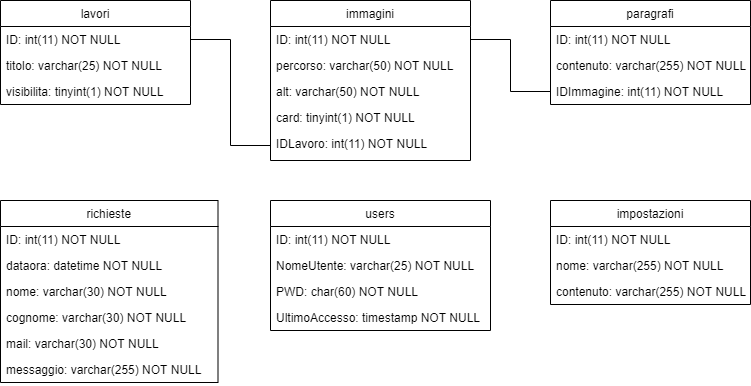
\includegraphics[scale = 0.5]{../latex/images/db.png}\\[1.5cm]
\end{center}

\subsection{Struttura dei contenuti}
Il sito si sviluppa nelle sue due parti, ovvero \textit{lato cliente} per i clienti interessati alla fioreria e ai prodotti che essa offre, e \textit{lato admin} per gli amministratori che si occupano della gestione dei contenuti del sito della fioreria. 

\subsubsection{Lato cliente}
Vengono ora descritte e argomentate le pagine che compongono il sito nel \textit{lato cliente}.\\\\
\textbf{Pagine}\\
Il layout desktop del lato client si presenta con delle strutture condivise uguali per tutte le pagine e poi in quest'ultime vengono sviluppati i temi a cui fanno riferimento.
	\begin{itemize}
		\item \textbf{Home} \\In questa pagina di introduzione si può visualizzare una prima selezione dei lavori scelti ad hoc con i corrispondenti link per una visione più approfondita in caso di interesse.
		\item \textbf{Chi siamo}\\In questa pagina l'utente trova una descrizione del personale e della storia del negozio. La pagina si presenta con due banner speculari ognuno dei quali formato da una foto e da una descrizione corrispondente.
		\item \textbf{Lavori}\\In questa pagina l'utente trova una lista di tutti i lavori al momento realizzabili in negozio. La pagina si presenta con un layout a card, ognuna delle quali per un lavoro differente, che hanno come sfondo una foto raffigurante il lavoro che rappresentano.\\\textbf{Qui riesci a spiegare il discorso del sottomenù e le modalità per vedere un lavoro specifico?}
	 	\item \textbf{Contatti}\\In questa pagina il cliente trova tutte le informazioni per contattare il negozio, quali email, numero di telefono ed indirizzo, inoltre è disponibile un form per contattare direttamente il negozio.
 	\end{itemize}
\textbf{Strutture fondamentali}\\ 
In tutte le pagine del lato client sono presenti 3 strutture in comune che facilitano la navigazione tra le varie pagine e riassumono le informazioni più importanti del sito.
	\begin{itemize}
		\item \textbf{Header}\\Il layout desktop di questa struttura si sviluppa in orizzonatale e in esso troviamo il logo del negozio e di fianco ad esso sono presenti i link per raggiungere le altre pagine del sito. Il layout mobile invece compatta i link per la navigazione in un menù ad hamburger che si sviluppa in verticale.
		\item \textbf{Breadcrumb}\\In questa struttura si trova il percorso fatto dall'utente per arrivare nella pagina che sta visualizzando, ciò serve per non creare smarrimento agli utenti che navigano all'interno del sito.
		\item \textbf{Footer}\\In questa struttura sono riassunti i contatti principali del negozio, che troviamo anche nella pagina dei Contatti, inoltre sono prensenti i vari social media in cui è presente il negozio per rimanere sempre aggiornati sulle offerte e sugli eventi speciali.
 	\end{itemize}
 		
\subsubsection{Lato admin}
Come prima cosa è bene precisare che tutti gli admin inseriti hanno tutti gli stessi permessi sulla gestione del sito. Questo è stato fatto perchè attualmente non ci sono esigenze particolari e gli accessi vengono farti da un numero ristretto di persone fidate.\\
Ogni amministratore si collega alla pagina di login e si autentica con le credenziali personali. È stata implementata una variabile di \texttt{SESSION}, per poter evitare che terzi possano accedere alle pagine di amministrazione senza essersi autenticati.\\
Vengono ora descritte e argomentate le pagine che compongono il sito nel \textit{lato cliente}.\\\\
\textbf{Pagine}\\ Il layout desktop per l'amministratore presenta un menù laterale a destra con tutte le pagine dove esso si può muovere. È un'interfaccia molto semplice e intuitiva per favorire l'usabilità anche dell'utente non molto esperto.
	\begin{itemize}
		\item \textbf{Dashboard};\\In questa pagina l'amministratore vede le ultime richieste inviate dai clienti e può modificare gli orari di apertura del negozio. Si è deciso di dare la possibilità all'amministratore di modificare solo gli orari, poichè il numero di telefono, l'email e l'indirizzo non sono dati che cambiano spesso, come invece lo sono gli orari di apertura. Uno sviluppo futuro potrebbe essere proprio quello di aggiungere uno spazio per la modifica anche di queste informazioni.
		\item \textbf{Gestione richieste};\\In questa pagina l'amministratore può leggere tutte le richieste che i clienti inviano tramite il form presente nella pagina di contatti del sito principale. La pagina mostra una lista di richieste, dalla più recente alla meno recente, ed ognuna di essere  si può cliccare per mostrare il contenuto e poi chiudere, oppure la si può eliminare. Non è pensato per creare un thread di comunicazione all'interno di questa pagina: l'amministratore ricontatterà i clienti tramite i propri servizi di posta elettronica, e in questo viene facilitato, in quanto gli basta cliccare sopra all'indirizzo email, per fare in modo di aprire il proprio servizio di posta elettronica e di inviare un'email con oggetto "Risposta Fioreria all'Arco".		
		\item \textbf{Gestione categorie};\\dire le pagine che lo compongono e come funziona il tutto
	 	\begin{itemize}
 			\item Aggiungi categoria;\\qualcosa qualcosa
 			\item Modifica categoria;\\qualcosa qualcosa
 			\item Elimina categoria;\\qualcosa qualcosa
	 	\end{itemize}
 	\item \textbf{Gestione utenti}\\In questa pagina l'amministratore autenticato può visionare gli account degli altri amministratori, eliminarne o aggiungerne uno di nuovo. 
 	\item \textbf{Logout}\\Quando l'amministratore clicca su questa voce del menù, effettua il logout dalla piattaforma e viene reindirizzato alla pagina di login. La variabile di \texttt{SESSION} viene quindi chiusa e quindi se l'amministratore prova ad accedere ad una specifica pagina di amministrazione dopo aver fatto il logout, viene reindirizzato alla pagina di login per potersi autenticare.\\
 	\end{itemize}
\textbf{Strutture fondamentali}
\begin{itemize}
	\item \textbf{Breadcrumb}\\	È stata inserita una breadcrumb in ogni pagina per aiutare l'utente a capire dove si trova. 
	\item \textbf{Funzionamento PHP}\\	DbConnection ecc.
\end{itemize}
